\documentclass{article}
\usepackage[utf8]{inputenc}
\usepackage[english]{babel}
\usepackage[T1]{fontenc}
\usepackage{graphicx}
\usepackage{siunitx}
\usepackage{xcolor}
\usepackage{float}
\usepackage{amsmath}
\usepackage[colorlinks=true, allcolors=blue]{hyperref}
\usepackage{caption}
\usepackage{subcaption}
\usepackage{minted}
\usepackage{verbatim}
\usepackage{framed}
\usepackage[a4paper, top=2.54cm, bottom=2.54cm, left=2.54cm, right=2.54cm, marginparwidth=1.75cm]{geometry}
\usepackage[style=ieee]{biblatex}
\addbibresource{../bibliography.bib}
\usepackage{csquotes}

\definecolor{backcolor}{rgb}{0.90,0.90,0.90}

%Use this environment for code that spans multiple pages
\newenvironment{longlisting}{\captionsetup{type=listing}}{}

\usemintedstyle{
    frame=lines,
    framesep=2mm,
    baselinestretch=1.2,
    bgcolor=backcolor,
    fontsize=\footnotesize,
    linenos
}

\begin{document}

\begin{centering}

{\scshape\Large {Junior Design II (Winter 2021)} \par}
\vspace{2cm}

{\huge\textit{Chicken Coop Monitoring System Developer Guide} \par}
\vspace{.5cm}

{\large{Austin Goergen}\par}
{\large{Alyssa Estenson}\par}
{\large{Bryson Goto}\par}
{\large{Ali Mohamed Alhabshi}\par}
\vspace{3cm}

\vspace{.3cm}


\end{centering}

\pagebreak

\section{System Overview}
The smart chicken coop monitoring system provides the user with an easier experience when taking care of chickens with its food and water monitoring system, autonomous heat lamp control, and warning lights for user intervention. Using real time clocks, as well as ultrasonic and daylight tracking sensors, the system is able to track the food and water levels, adjust the heat lamp for the chickens depending on the time of day, as well as warn the user if the resource levels are too low. All of this data is logged to an SD card, allowing the user to check the coop's conditions for several weeks.
\section{Electrical Specifications}

\begin{figure}[H]
    \centering
    \includegraphics[width=\textwidth]{fig/electrical-chars-1.pdf}
    \caption{First table of electrical characteristics}
    \label{fig:electric-char-1}
\end{figure}

\begin{figure}[H]
    \centering
    \includegraphics[width=\textwidth]{fig/electrical-chars-2.pdf}
    \caption{Second table of elecrical characteristics}
    \label{fig:electric-char-2}
\end{figure}


\section{User Guide}
\subsection{Initial Setup}
To begin setup of the chicken coop monitoring system, start by connecting the external warning lights, food sensor, water sensor, and heat lamp to the appropriate connectors shown in figure \ref{fig:front-connector}.  The daylight sensor comes pre-installed in the system enclosure and must remain unobstructed in order to work properly.

\begin{figure}[H]
    \centering
    \includegraphics[width=\textwidth]{fig/panel-labels.png}
    \caption{Front connector labels}
    \label{fig:front-connector}
\end{figure}

The food and water sensors are ultrasonic sensors that detect how far away the food or water is.  They should be positioned directly above the food or water without any additional obstructions in front of them as shown in figure \ref{fig:sensor-setup}.

\begin{figure}[H]
    \centering
    \includegraphics[width=\textwidth]{fig/sensor-setup.jpg}
    \caption{Food and water sensor setup}
    \label{fig:sensor-setup}
\end{figure}

The chicken coop monitoring system can use any heat lamp with a NEMA 5-15P connector.  The heat lamp can be plugged into either of the electrical outlets connected to the system.  If desired, two smaller heat lamps can be used instead as long as their combined power draw is no more than 180 watts.

After connecting all external sensors and lights, an SD card must be inserted into the SD card slot shown in figure \ref{fig:sd-card-location} so that the system can log data.  Note that the SD card can be removed at any time during system operation.

\begin{figure}[H]
    \centering
    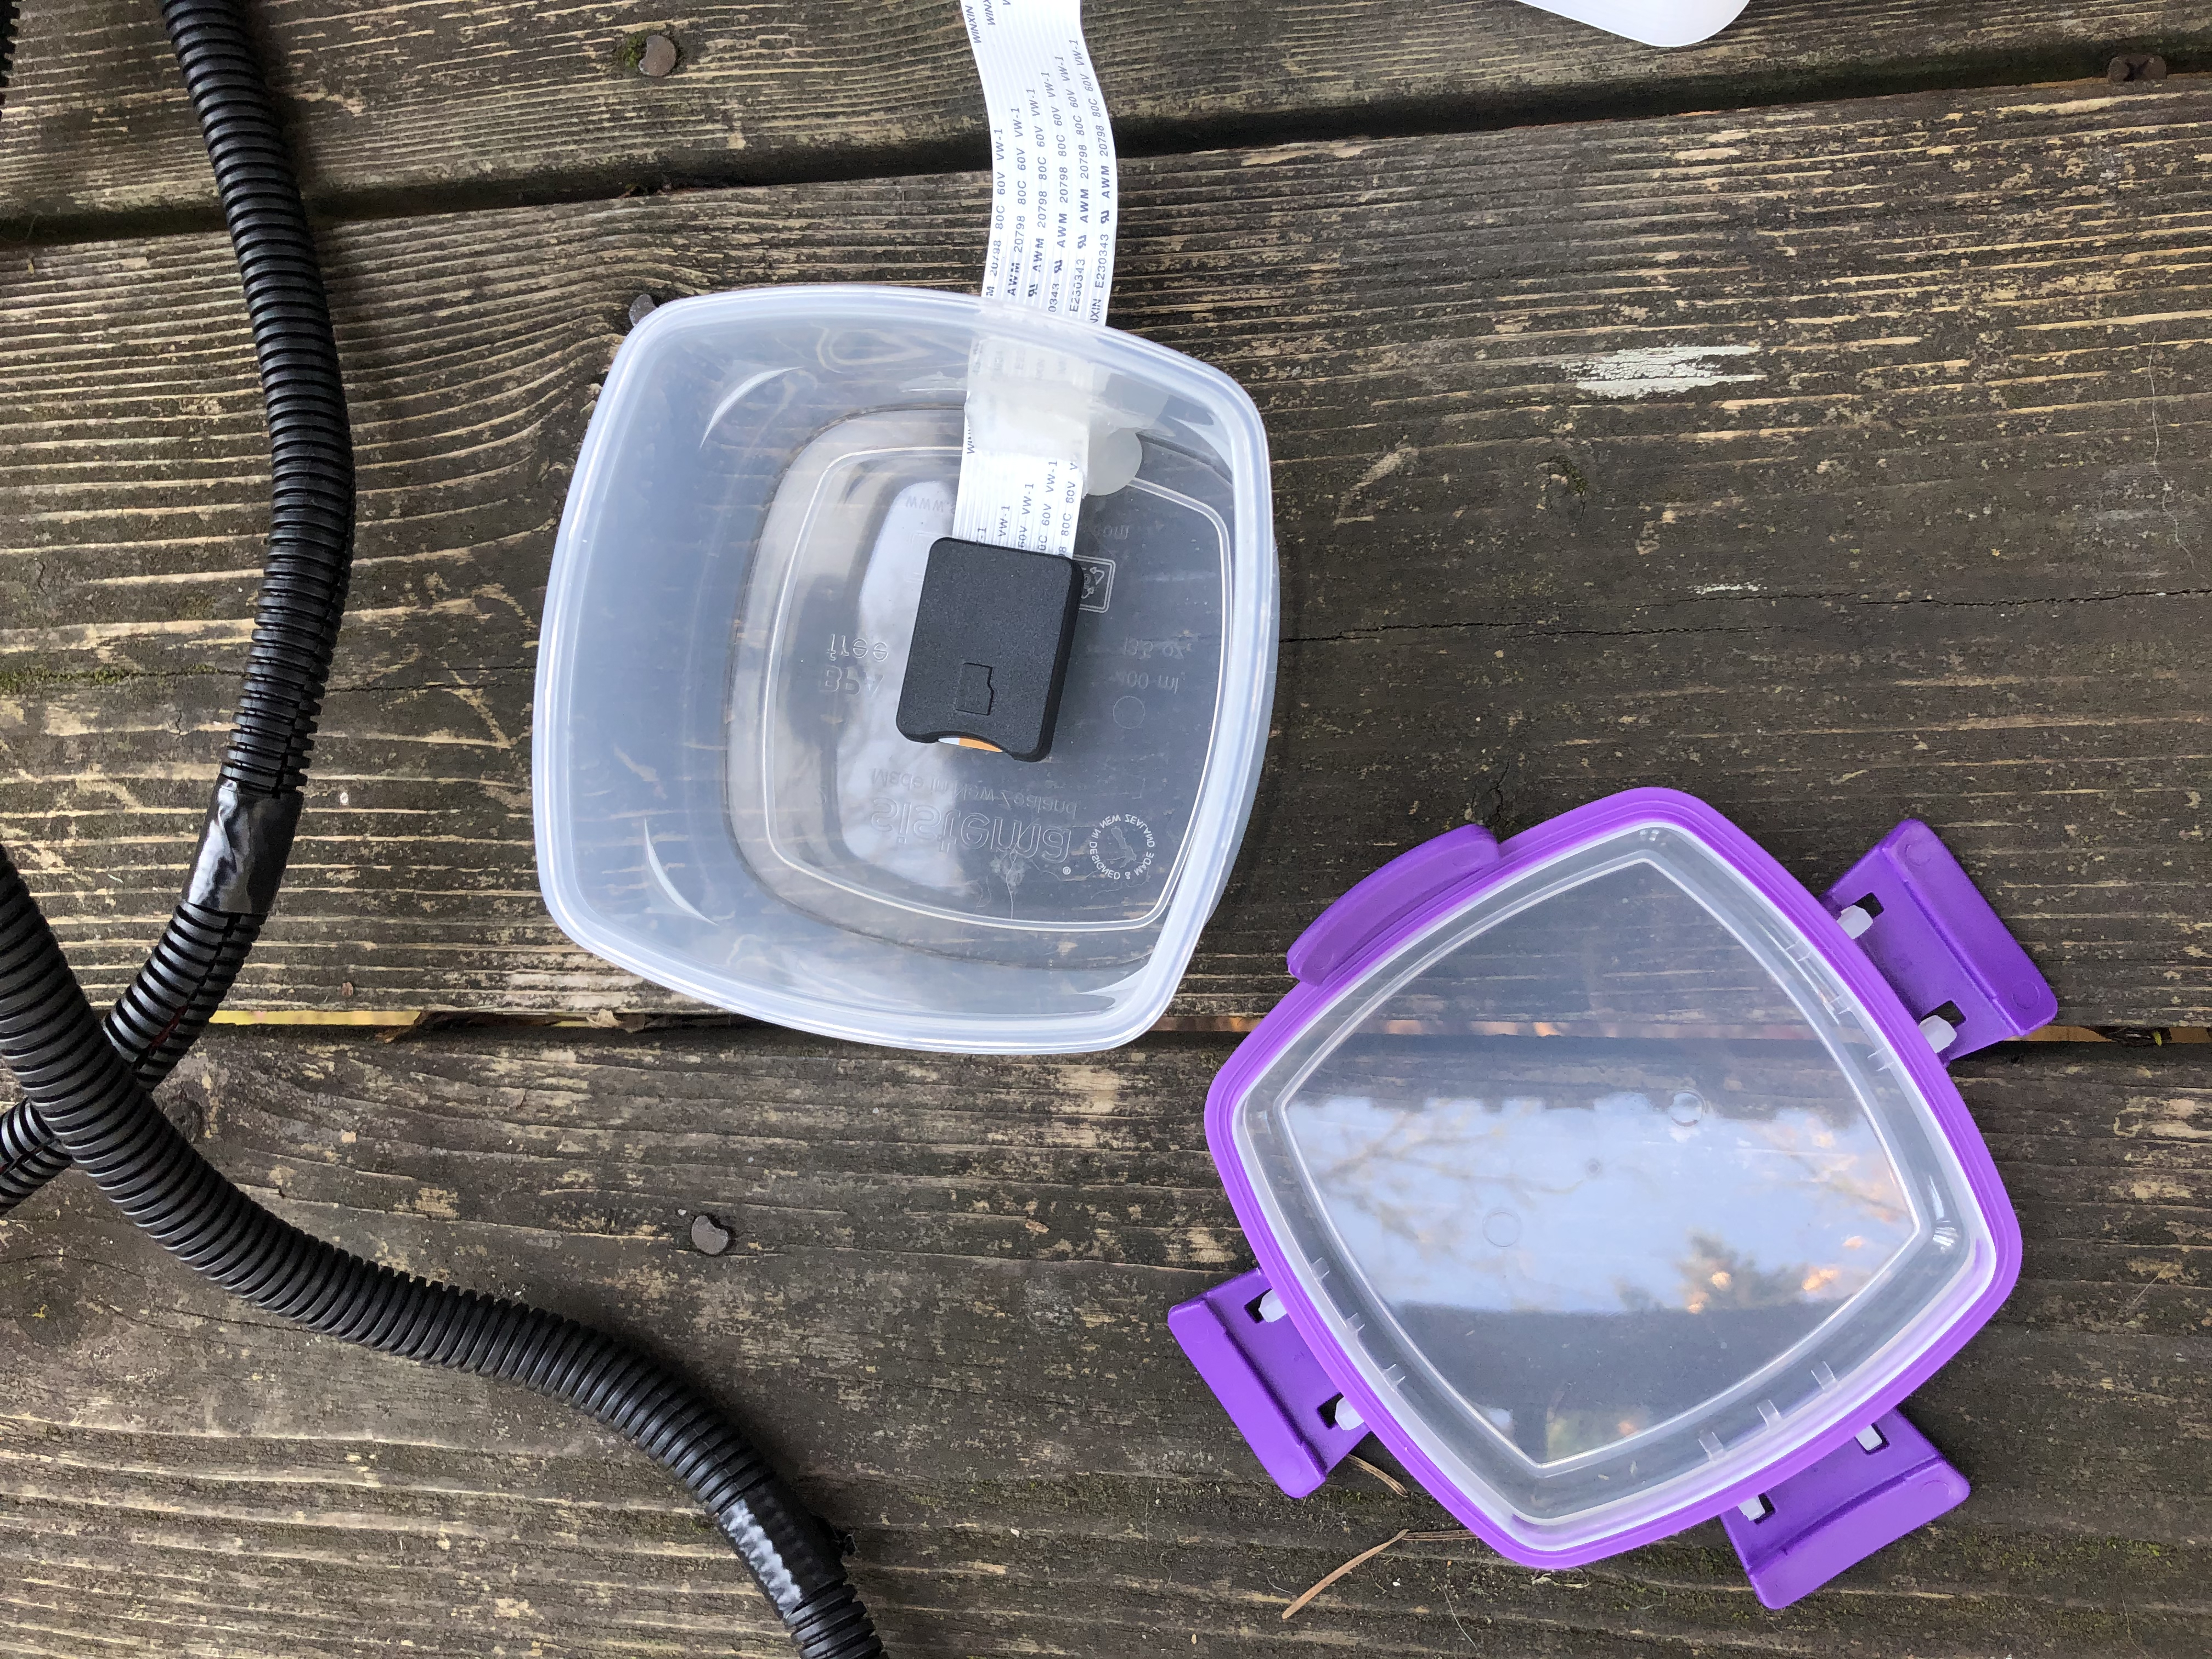
\includegraphics[width=\textwidth]{fig/sd-setup.jpg}
    \caption{SD card location}
    \label{fig:sd-card-location}
\end{figure}

\subsection{Booting Up the System}
The system is powered using a C13 power cord.  Plug one end of the chord into a wall outlet and the other end into the chicken coop monitoring system.  Flip the power switch and verify that a red light is illuminated under the switch.

The system will perform its initialization sequence after the power switch is flipped.  The system will turn the heat lamp on full power and turn on each warning light for a short period of time to verify they are connected properly.  The system is now monitoring and logging food and water levels, determining if any warning lights need to be turned on, and tracking time to determine when the heat lamp should be turned on or dimmed.

\subsection{Interpretting Warning Lights and Heat Lamp Behavior}
The Chicken Monitoring System utilizes a signal tower with three lights triggered at different conditions. The following conditions signal when resources are stable, or require attention for refill. Specifically, the lights represent the following, in order from top to bottom on the tower:

\begin{itemize}
    \item Red: Food is below 20\% of full capacity, and requires a refill.
    \item Yellow: Water is below 20\% of full capacity, and requires a refill.
    \item Green: All resources are at a sufficient level.
\end{itemize}

Note that if multiple resources require attention, both the red and yellow lights may trigger. Once the system detects the resources are filled to a higher capacity, the red and/or yellow lights will shut off. If resources no longer require attention, the green light should always be on.

The heat lamp attached to the system is controlled by the time of day. In order to account for both the lowering temperature and loss of daylight, the heat lamp is set to turn on at 3:00pm. To consistently provide 14 hours of light for the chicken coop, the time period most optimal for laying eggs, the heat lamp is set to begin its shutdown sequence at 9:00pm. The sequence lasts 10 minutes, dimming to one of five discrete brightness levels every 2 minutes. This provides time for chickens to return to their roosting stick.

\subsection{Viewing Logged Data}
The data logged for resource consumption and daylight hours over the past two weeks is automatically written to the SD card while it is connected to the system. In order to see this information logged onto a graph, you may eject the SD card at any time, without needing to reboot the system.

Once the SD card is ejected from it’s extender module, insert the SD card into your computer. The file containing the resource and daylight data is a type .csv, titled “TEST.” This is the only file on the SD card the enclosure interacts with.

Once locating this file, locate the MATLAB Code file titled “JD\_SCRIPT.” Copy the “TEST.csv” file to the same directory where “JD\_SCRIPT” is located. Open the file in MATLAB, run the script, and a figure showing the data should appear, similar to the one below in Figure GRAPH.

\begin{figure}[H]
    \centering
    \includegraphics[width=\textwidth]{fig/example-graph.png}
    \caption{Example graph after filling food and water}
    \label{fig:example-graph}
\end{figure}

When the SD card is reinserted into the system after viewing, data will automatically continue to be updated to the card. However, note that for any measurement period where the card is not present in the system, the measured data will not be logged. If desired, the “TEST” file may be deleted at any time on the SD card, and the system will simply create another.
\newpage

\section{Design Artifact Figures}

\begin{figure}[H]
    \centering
    \includegraphics[width=\textwidth]{fig/block-diagram.pdf}
    \caption{Complete block diagram of the chicken coop monitoring system.}
    \label{fig:block-diagram}
\end{figure}

\begin{figure}[H]
    \centering
    \includegraphics[width=\textwidth]{fig/schematic.pdf}
    \caption{Complete schematic of the chicken coop monitoring system.  The entire system is powered from a single 120 VAC wall outlet and uses a custom PCB to connect external sensors to the Arduino Nano.  This schematic also shows which conductors of the waterproof Conxall connectors are used.}
    \label{fig:schematic}
\end{figure}

% interface definitions
% 3d model
\section{PCB Information}
\section{Part Information}
\end{document}